\documentclass[a4paper,12pt]{article}
%spellchecker
% !TeX spellcheck = de

\usepackage{amssymb} % needed for math
\usepackage{amsmath} % needed for math
\usepackage[utf8]{inputenc} % this is needed for german umlauts
\usepackage[ngerman]{babel} % this is needed for german umlauts
\usepackage[T1]{fontenc}    % this is needed for correct output of umlauts in pdf
\usepackage[margin=2.5cm]{geometry} %layout
\usepackage{booktabs}



% this is needed for forms and links within the text
\usepackage{hyperref}  

% Generate the glossary
\usepackage[nonumberlist]{glossaries}
\makeglossary

% The following is needed in order to make the code compatible
% with both latex/dvips and pdflatex.
\ifx\pdftexversion\undefined
\usepackage[dvips]{graphicx}
\else
\usepackage[pdftex]{graphicx}
\DeclareGraphicsRule{*}{mps}{*}{}
\fi

%%%%%%%%%%%%%%%%%%%%%%%%%%%%%%%%%%%%%%%%%%%%%%%%%%%%%%%%%%%%%%%%%%%%%%
% Variablen                                 						 %
%%%%%%%%%%%%%%%%%%%%%%%%%%%%%%%%%%%%%%%%%%%%%%%%%%%%%%%%%%%%%%%%%%%%%%
\newcommand{\authorName}{Lena Gregor, Dominik Horn}
\newcommand{\auftraggeber}{Lehrstuhl für Datenbanksysteme TUM}
\newcommand{\auftragnehmer}{\authorName}
\newcommand{\projektName}{Wahl und Informationssystem für bayrische Landtagswahlen}
\newcommand{\tags}{\authorName, Pflichtenheft, TUM, Universität Augsburg, LMU}
\newcommand{\subtitle}{Technische Universität München, Datenbanksysteme WS19/20}
\newcommand{\glossarName}{Glossar}

%%%%%%%%%%%%%%%%%%%%%%%%%%%%%%%%%%%%%%%%%%%%%%%%%%%%%%%%%%%%%%%%%%%%%%
% PDF Meta information                                 				       %
%%%%%%%%%%%%%%%%%%%%%%%%%%%%%%%%%%%%%%%%%%%%%%%%%%%%%%%%%%%%%%%%%%%%%%
\hypersetup{
  pdfauthor   = {\authorName},
  pdfkeywords = {\tags},
  pdftitle    = {\projektName~(Pflichtenheft)}
} 

%%%%%%%%%%%%%%%%%%%%%%%%%%%%%%%%%%%%%%%%%%%%%%%%%%%%%%%%%%%%%%%%%%%%%%
% Custom setup                                                       % 
%%%%%%%%%%%%%%%%%%%%%%%%%%%%%%%%%%%%%%%%%%%%%%%%%%%%%%%%%%%%%%%%%%%%%%
\usepackage{pdfpages}
\usepackage{xcolor,colortbl} 
\definecolor{Blue}{rgb}{0.1,0.2,0.7}
\definecolor{TUMBlue}{HTML}{0065BD}
\definecolor{TUMSecondaryBlue}{HTML}{005293}
\definecolor{TUMSecondaryBlue2}{HTML}{003359}
\definecolor{TUMAccentBlue}{HTML}{64A0C8}
\definecolor{TUMAccentLightBlue}{HTML}{98C6EA}
\definecolor{lightBlue}{RGB}{157,195,230}


\newcolumntype{a}{>{\columncolor{TUMBlue}}c}
\newcolumntype{b}{>{\columncolor{lightBlue}}c}

\renewcommand{\arraystretch}{1.5}
 
%%%%%%%%%%%%%%%%%%%%%%%%%%%%%%%%%%%%%%%%%%%%%%%%%%%%%%%%%%%%%%%%%%%%%%
% Create a shorter version for tables. DO NOT CHANGE               	 %
%%%%%%%%%%%%%%%%%%%%%%%%%%%%%%%%%%%%%%%%%%%%%%%%%%%%%%%%%%%%%%%%%%%%%%
\newcommand\addrow[2]{\textcolor{black}{#1} &#2\\ \hline}

\newcommand\addheading[2]{\rowcolor{TUMBlue}\textcolor{white}{#1} & \textcolor{white}{#2}\\ \hline}
\newcommand\tabularhead{\begin{tabular}{|b|p{13cm}|}
\hline
}

\newcommand\addmulrow[2]{ \begin{minipage}[t][][t]{2.5cm}#1\end{minipage}% 
   &\begin{minipage}[t][][t]{8cm}
    \begin{enumerate} #2   \end{enumerate}
    \end{minipage}\\ }

\newenvironment{usecase}{\tabularhead}
{\hline\end{tabular}}

%%%%%%%%%%%%%%%%%%%%%%%%%%%%%%%%%%%%%%%%%%%%%%%%%%%%%%%%%%%%%%%%%%%%%%
% THE DOCUMENT BEGINS             	                              	 %
%%%%%%%%%%%%%%%%%%%%%%%%%%%%%%%%%%%%%%%%%%%%%%%%%%%%%%%%%%%%%%%%%%%%%%
\begin{document}
 \pagenumbering{roman}
 \begin{titlepage}
\maketitle
\thispagestyle{empty} % no page number

\begin{verbatim}












\end{verbatim}


  \begin{tabular}[t]{ll}
	Projekt:       & \quad \projektName \\[1.2ex]
	Auftraggeber:  & \quad \auftraggeber\\[1.2ex]
	Auftragnehmer: & \quad \auftragnehmer\\[1.2ex]
  \end{tabular}

\begin{tabular}{|p{3 cm}|p{3 cm}|p{5 cm}|}
\hline
\textbf{Version} & \textbf{Datum} & \textbf{Autor(en)} \\
\hline
\hline
1.0 & 04.11.2019 & \authorName \\
\hline
\end{tabular}
\end{titlepage}
         % Deckblatt.tex laden und einfügen
 \setcounter{page}{2}

 \tableofcontents          % Inhaltsverzeichnis ausgeben
 \clearpage
 \pagenumbering{arabic}
 
\section{Zielbestimmung}
%%%%%%%%%%%%%%%%%%%%%%%%%%%%%%%%%%%%%%%%%%%%%%%%%%%%%%%%%%%%%%%%%%%%%%
% Warum wird das Projekt gemacht?           						 %
%%%%%%%%%%%%%%%%%%%%%%%%%%%%%%%%%%%%%%%%%%%%%%%%%%%%%%%%%%%%%%%%%%%%%%
Der Freistaat Bayern möchte in Kooperation mit dem Lehrstuhl für 
Datenbanksysteme an der Technischen Universität München eine digitales 
Wahlinformations- und Stimmabgabesystem für Landtagswahlen mithilfe von 
Studierenden des Elite Software Engineering Masterstudiengangs aufbauen.
%
Das System soll dabei nicht nur die Ergebnisse für die Landtagswahlen 
2013 und 2018 analysier- und vergleichbar machen, e.g., die Sitzverteilung 
im Landtag, statistische Auswertung von Ergebnissen, Berechnung gewonnener
Mandate, sondern auch als sicheres Backendsystem für die elektronische 
Stimmabgabe im Wahllokal dienen. 
%
Es müssen die gesetzlichen Regelungen, Normen und Datenschutzaspekte
berücksichtigt werden. Als Basis gelten die Regelungen zur
Landtagswahl 2018


\subsection{Musskriterien}
% Requirements
\begin{usecase}
	\addheading{Nummer}{Die Anwendung ermöglicht es...} 
	\addrow{M1}{...dem Wähler Einzelstimmen abzugeben nachdem die Stimmabgabe durch den Wahlhelfer freigegeben wurde.}
	\addrow{M2}{...dem Wahlhelfer Stimmen aggregiert einzugeben.}
	\addrow{M3}{...Daten von vergangenen Wahlen mit Hilfe einer CSV-Datei fehlerfrei in das System einzuspeisen und statistisch auszuwerten.}
	\addrow{M4}{...bei der statistischen Auswertung die Verteilung der Sitze, die Auswertung für die Direkt- und Listenmandate, Anzahl Stimmen pro Partei einzusehen}
	\addrow{M5}{...pro Stimmkreis die Einzelstimmen zu Stimmkreisergebnissen vorzuaggregieren.}
	\addrow{M6}{...dass 10 Personen in einem Wahllokal gleichzeitig auf das System zugreifen und ihre Stimme eintragen.}
	\addrow{M7}{...Stimmabgaben als gültig und ungültig auszuwerten.}
	\addrow{M8}{...erst nach Abschluss einer Wahl diese statistisch Auswzuwerten, um Wahlbeeinflussung zu verhindern.}
	\addrow{M9}{...Wahlleitern, schon eingegebene Stimmen noch einmal zu korrigieren, beispielsweise nach einer Neuauszählung}
	\addrow{M10}{Die Anwendung speichert Erst- und Zweitstimmen getrennt voneinander.}
	\addrow{M11}{Die Oberfläche zur statistischen Auswertung ist frei zugänglich, die zur Stimmabgabe (durch Wähler oder Wahlhelfer/ -leiter) je nur für Berechtigte.}
	
\end{usecase}

\subsection{Sollkriterien}
\begin{usecase}
	\addheading{Nummer}{Beschreibung} 
	\addrow{S1}{Die Anwendung ermöglicht es dem Anwender die Ergebnisse von unterschiedlichen Wahlen zu vergleichen.}
\end{usecase}
\subsection{Kannkriterien}
\begin{usecase}
	\addheading{Nummer}{Beschreibung} 
	\addrow{K1}{Die Anwendung kann bei der statistischen Auswertung die Ergebnisse auf der Landkarte visualisieren}
\end{usecase}

\subsection{Abgrenzungskriterien}
\begin{usecase}
	\addheading{Nummer}{Beschreibung} 
	\addrow{A1}{Die Anwendung ermöglicht nicht die Authentifizierung von Wahlberechtigten.}
	\addrow{M2}{Die Anwendung verarbeitet/ berechnet keine juristischen Ausnahmefälle, die bei den Wahlen 2013 und 2018 nicht relevant waren.}
	
\end{usecase}


\section{Technische Umsetzung}
Dieser Abschnitt widmet sich der geplanten technischen Realisierung
aller Systemaspekte.

\subsection{Produkteinsatz und Umgebung}
Die Anwendung ist konzipiert und entwickelt um die Stimmabgabe 
zu bayrischen Landtagswahlen (Erst-, Zweitstimme) durch wahlberechtigte
Personen, sowie die (statistische-) Auswertung von Wahlergebnissen zu ermöglichen. 
%
Das System wird in verschiedenen Gebieten eingesetzt:

\begin{center}
\begin{tabular}{|m{5cm}|m{10cm}|}
	\hline
  \rowcolor{TUMBlue} \textcolor{white}{\textbf{Einsatzgebiet}} & \textcolor{white}{\textbf{Prozesse}} \\
  \hline
  Wahllokal & Abgabe von Einzelstimmen durch WählerInnen und batch Stimmeintragung durch WahlhelferInnen \\
	\hline
  Bürgerlicher Gebrauch & (statistische-)Analyse von Wahlergebnissen \\
  \hline
  Staatlicher Gebrauch & (statistische-)Analyse von Wahlergebnissen, Import von alten Wahlergebnissen \\
	\hline
\end{tabular}
\end{center}

Die (statistische-) Analyse und Auswertung von Wahlergebnissen erfolgt in einer frei zugänglichen
Weboberfläche, welche auf ein Serversystem zur Datenbeschaffung zugreift. 
Während eines Wahlvorgangs sind Daten zum aktuellen Vorgang nicht (statistisch-) Auswertbar.
%
Das Wahlinterface sowie die von WahlhelferInnen und WahlleiterInnen zu benutzenden Oberflächen sind 
ebenfalls mit Webtechnologien implementiert, jedoch Zugriffbeschränkt und nicht übers Internet aufrufbar.
%
Webtechnologien für alle Interfaces zu verwenden senkt den Projektaufwand, da Entwickler sich nur in 
einem Technologiestack bewegen müssen. Weiterhin sind insbesondere Webtechnologien dafür geeignet
Geräte und bildschirmgrößen-unabhängige Software zu erzeugen.
%
Jede Personengruppe kann zu jeder Zeit immer nur auf die für sie relevanten Interfaces zugreifen.
Dies steigert primär die intuitive Benutzbarkeit und verhindert Benutzern zu verwirren. 
%
Als Backendsystem wird ein zugriffsgesichertes DBMS eingesetzt. Dieses implementiert mehrere 
essentielle Projektbestandteile out-of-the-box:

\begin{itemize}
      \item Parallele OLAP Abfragen, i.e., mehrere Benutzer können gleichzeitig ungehindert voneinander 
            die Wahlergebnisse statistisch auswerten.
      \item Mehrbenutzer OLTP, i.e., mehrere WählerInnen und WahlhelferInnen können parallel Stimmen
            eintragen.
      \item Hohe Ausfallsicherheit, i.e., das System läuft stabil über längere Zeiträume
      \item Recovery Funktionalität, i.e., falls ein Unglück geschieht (Brand im Datencenter, Stromausfall) 
            oder das DBMS abstürzt gehen keine Daten verloren, solange die entsprechenden DBMS features 
            genutzt werden
      \item Datenzugriffschnittstelle ist standartisiert und flexibel (SQL)
      \item Integritätsbedingungen werden über das Datenbankschema automatisch realisiert
\end{itemize}

\subsection{Eingesetzte Technologien}
Nachfolgend wird für jedes Einsatzgebiet die eingesetzte Technologie zusammen mit einer kurzen Erläuterung
für Ihren Einsatz aufgelistet.

\begin{center}
      \begin{tabular}{|m{3cm}|m{3cm}|m{9cm}|}
            \hline
        \rowcolor{TUMBlue} \textcolor{white}{\textbf{Gebiet}} & \textcolor{white}{\textbf{Eingesetzte Technologie}} & \textcolor{white}{\textbf{Erläuterung}} \\
        \hline
        Programmier- sprache & TypeScript & TypeScript ist eine von Microsoft entwickelte Programmiersprache, welche JavaScript hauptsächlich um statische Typisierungsfähigkeiten ergänzt. Sie ist die Implementierungssprache für alle Softwarebereiche dieses Projekts \\
        \hline
        Backend DBMS & PostgreSQL & PostgreSQL ist ein von der Industrie großflächig eingesetztes kostenfreies DBMS mit sehr guter Reputation und erprobtem Produktiveinsatz in großen Anwendungen \\
        \hline
        Backend Server & NodeJS & NodeJS ermöglicht es Plattformunabhängig JavaScript code auszuführen. Hier dient es dazu die Serversoftware auszuführen \\
        \hline
        Backend Server & Apollo Server & Apollo Server implementiert die notwendige serverseitige Funktionalität um auf GraphQL Anfragen zu antworten. Jeder request wird auf einen resolver-Funktion gemapped, welche sich darum kümmert die angeforderte funktion (Daten lesen, Daten schreiben) auszuführen. \\
        \hline
        Frontend Server Schnittstelle & Apollo Client & Apollo Client implementiert die notwendige clientseitige Funktionalität um GraphQL Anfragen an einen Server zu schicken und die Antworten zu empfangen \\
        \hline
        Frontend UI & React & React ist ein von Facebook entwickeltes UI-Framework und wird zur Darstellung sämmtlicher Inhalte verwendet \\
        \hline
        Frontend UI & Ant Design & Ant Design ist eine React Component Library, welche viele nützliche GUI-Elemente vorgefertigt bereitstellt \\
        \hline
      \end{tabular}
\end{center}

\subsection{Umsetzung der Muss- und Sollkriterien}
% Wie genau werden die ganzen Muss/Soll kriterien erfüllt

\section{GUI Mockups}

\section{Datenmodell}
Die grundlegenden zu verwaltenden Produktdaten ergeben sich aus der folgenden Liste von
identifizierten Entitäten:
\begin{itemize}
  \item \textbf{Wahl} - Repräsentation einer einzelnen Wahl an einem festen Datum. 
        Durch letzteres Merkmal ist es möglich mehrere Wahlen in einem Jahr festzuhalten.
  \item \textbf{Stimme} - Jede(r) WählerIn besitzt je eine Erst- und Zweitstimme, welche er oder sie in Ihrem
        Stimmbezirk für KandidatInnen abgeben können. Mit der Erststimme wählt eine wahlberechtigte Person
        primär den oder die von ihr bevorzugten DirektkandidatIn ihres Stimmkreises. Über die Zweitstimme wählt 
        jede wahlberechtigte Person genau einen Kandidaten einer Liste aus ihrem Regierungsbezirk. Das prozentuale
        Gesamtabschneiden einer Partei aus kombinierten Erst- und Zweitstimmen ist jedoch ebenso für das 
        Wahlergebnis relevant.
  \item \textbf{Regierungsbezirk} - Bayern ist in sieben Regierungsbezirke unterteilt: Oberbayern,
        Niederbayern, Schwaben, Ober-, Unter-, Mittelfranken und Oberpfalz. Jeder Regierungsbezirk
        hat eine unterschiedliche Anzahl zu vergebender Direkt- und Listenmandate
  \item \textbf{Stimmkreis} - Regierungsbezirke sind gemäß Bevölkerungszahlen in Stimmkreise aufgeteilt.
        Jeder Stimmkreis ist widerum in ein oder mehrere Stimmbezirke unterteilt. Pro Stimmkreis wird ein(e)
        DirektkandidatIn gewählt
  \item \textbf{Stimmbezirk} - Die Stimmabgabe erfolgt in Stimmbezirken
  \item \textbf{KandidatIn} - Eine sich zur Wahl stellende Person mit notwendigen persönlichen Angaben. 
        Insbesondere kann ein(e) KandidatIn als DirektkandidatIn für einen Stimmkreis aufgestellt sein.
  \item \textbf{Mandat} - Mandate für den Bayrischen Landtag können von KandidatInnen im Rahmen einer Landtagswahl
        errungen werden. Hierbei wird zwischen Direktmandaten, Listenmandaten und Ausgleichsmandaten unterschieden.
  \item \textbf{Partei} - KandidatInnen können Mitglied einer Partei sein und sich von dieser für einen Listenplatz
        aufstellen lassen
  \item \textbf{Liste} - Jede Partei kann pro Regierungsbezirk eine Liste mit KandidatInnen, welche Mitglieder der 
        Partei sind, aufstellen.
\end{itemize}

\begin{center}
	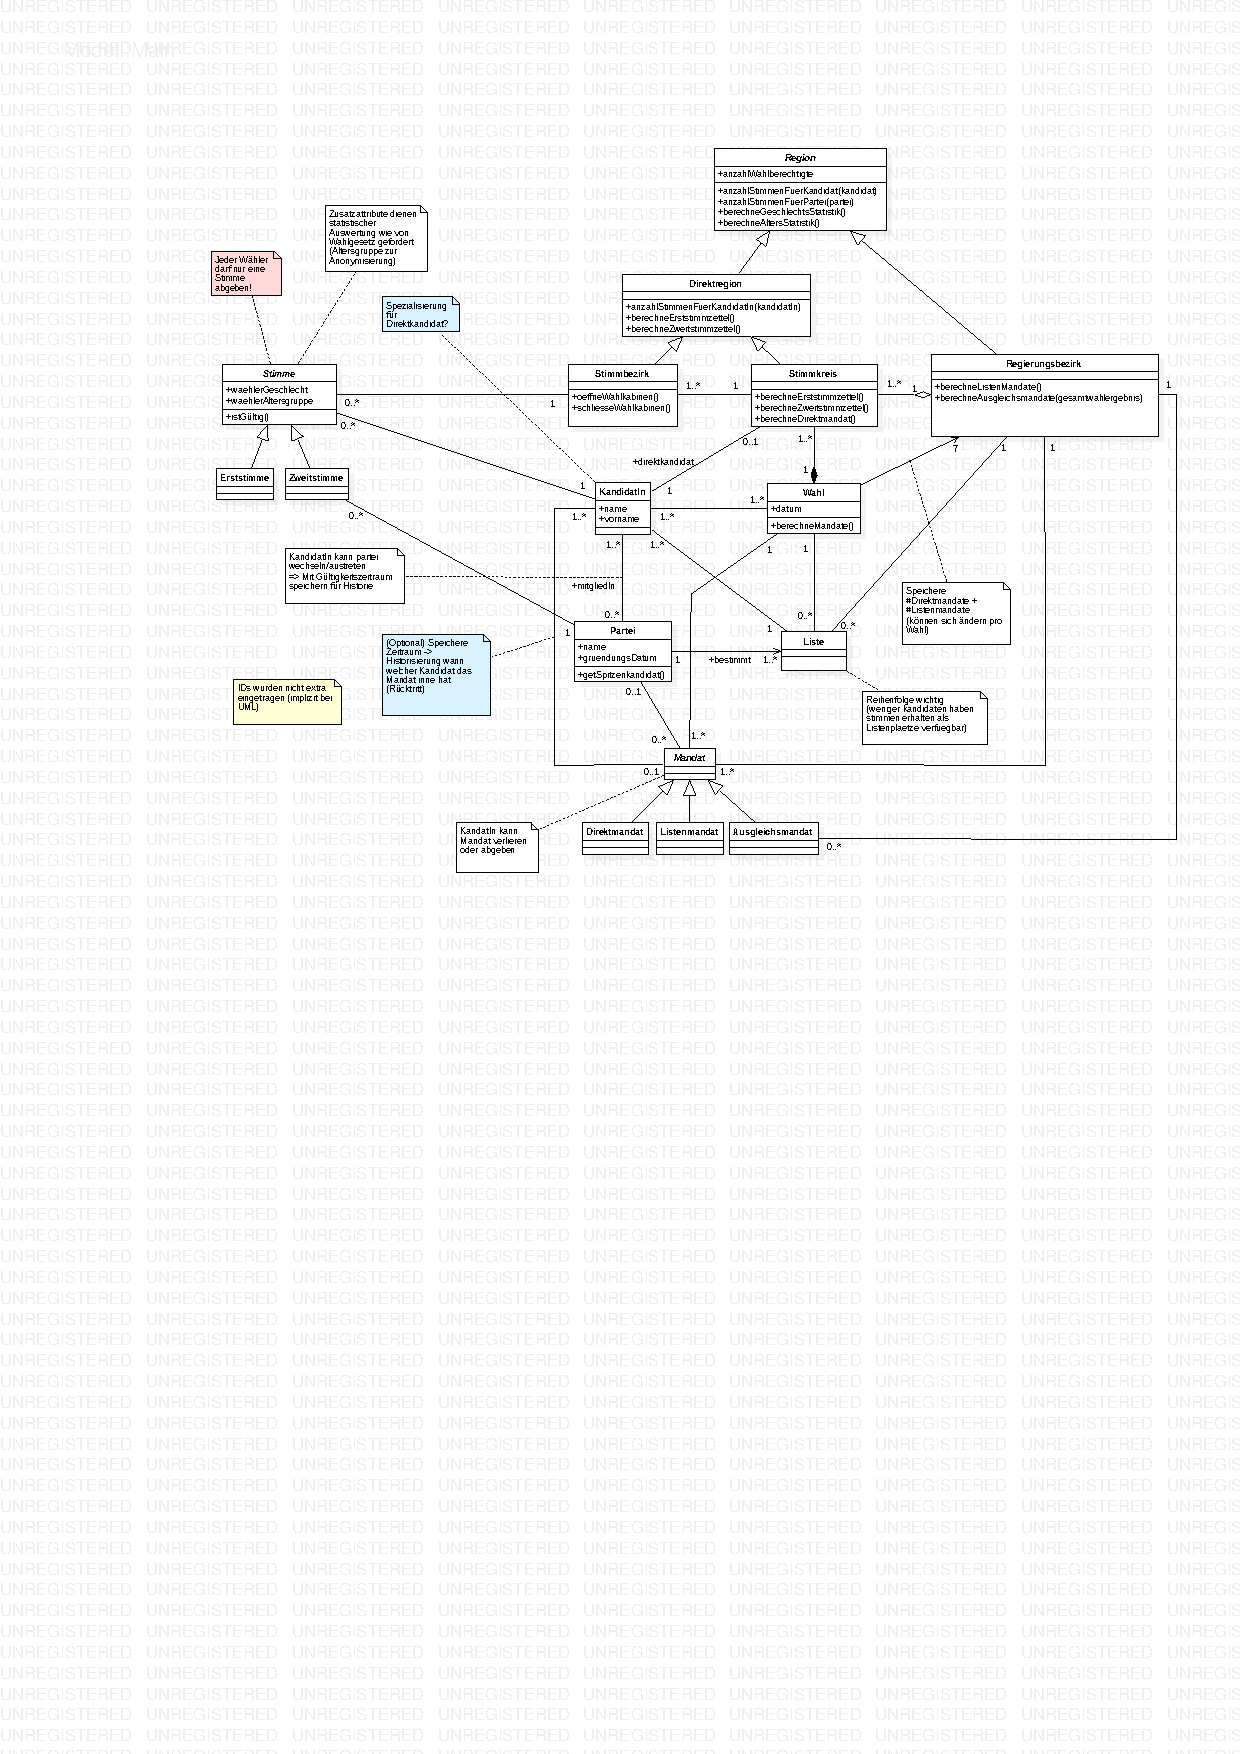
\includegraphics[width=\textwidth]{../model.pdf}
\end{center}

\section{Globale Testfälle und Szenarien}
% 10 Leute gleichzeitig in Wahllokal greifen zu
% Auswertung realer wahlergebnisse geht flott

\clearpage
%%%%%%%%%%%%%%%%%%%%%%%%%%%%%%%%%%%%%%%%%%%%%%%%%%%%%%%%%%%%%%%%%%%%%%
% Begriffslexikon zur Beschreibung des Produkts						 %
%%%%%%%%%%%%%%%%%%%%%%%%%%%%%%%%%%%%%%%%%%%%%%%%%%%%%%%%%%%%%%%%%%%%%%
%\newglossaryentry{sortierschluessel}
%{
%  name=Sortierschlüssel,
%  description={ein Schlüssel, anhand dessen diese Einträge sortiert werden}
%}
\newglossaryentry{Technologiestack}
{
  name=Technologiestack,
  description={Sammlung aller verwendeten Technologien im Projekt. Gegebenenfalls hierarchisch sortiert wenn aufeinander aufbauend}
}
\newglossaryentry{Client}
{
  name=Client,
  description={Programm, dass die Dienste eines Servers in Anspruch nimmt}
}
\newglossaryentry{Server}
{
  name=Server,
  description={Rechner, der für andere in einem Netzwerk mit ihm verbundene Systeme bestimmte Aufgaben übernimmt und von dem diese ganz oder teilweise abhängig sind}
}
\newglossaryentry{Datenbanksystem}
{
  name=Datenbanksystem,
  description={Ein Datenbanksystem (DBS) ist eine systematisch strukturierte, langfristig verfügbare Sammlung von Daten einschließlich der zur Verwaltung notwendigen Software}
}
\newglossaryentry{OLAP}
{
  name=OLAP,
  description={Online Analytical Processing}
}
\newglossaryentry{OLTP}
{
  name=OLTP,
  description={Online Transaction Processing}
}


% Setze den richtigen Namen für das Glossar
\renewcommand*{\glossaryname}{\section{\glossarName}}

% Drucke das gesamte Glossar
\glsaddall
\printglossaries

% Trage das Glossar in das Inhaltsverzeichnis ein
\stepcounter{section}
\addcontentsline{toc}{section}{\numberline {\thesection} \glossarName}
\end{document}
